\documentclass[a4paper,12pt]{article}
\usepackage[utf8]{inputenc} % Required for inputting international characters
\usepackage[T1]{fontenc} % Output font encoding for international characters
\usepackage{float}
\usepackage{mathpazo} % Use the Palatino font by default
\usepackage[autostyle=true]{csquotes} % Required to generate language-dependent quotes in the bibliography
\usepackage{pdfpages}
\usepackage{amsmath}
\usepackage{subcaption}
\usepackage{xcolor}
\usepackage[square,numbers,sort]{natbib}
\usepackage{multirow}
\usepackage[newfloat]{minted} % Code listings, with syntax highlighting
\usepackage{caption}
\usepackage{tablefootnote} % for table footnotes
\usepackage{hyperref}
\usepackage[english]{babel}
\usepackage[useregional]{datetime2}
\usepackage[
    left = \flqq{},% 
    right = \frqq{},% 
    leftsub = \flq{},% 
    rightsub = \frq{} %
]{dirtytalk}
\usepackage{geometry}
\geometry{
	paper=a4paper, % Change to letterpaper for US letter
	inner=2.75cm, % Inner margin
	outer=3.5cm, % Outer margin
	bindingoffset=.5cm, % Binding offset
	top=2.5cm, % Top margin
	bottom=2.5cm, % Bottom margin
	%showframe, % Uncomment to show how the type block is set on the page
}
\usepackage{enumitem}
\usepackage{fdsymbol}
\usepackage{latexsym}
\usepackage{pdflscape}

\bibliographystyle{unsrtnat}

\newenvironment{code}{\captionsetup{type=listing}}{}
\SetupFloatingEnvironment{listing}{name=Código}

\hypersetup{
    colorlinks,
    linkcolor={red!80},
    citecolor={red!80},
    urlcolor={red!80}
}

\begin{document}

\pagenumbering{gobble} % remove page numbers (and reset to 1)

\newlist{dig}{itemize}{6}
\setlistdepth{6} 

% Configure the behaviour of levels entries
\setlist[dig, 1]
{label=$\medblacktriangleright$ , 
leftmargin=\parindent,
rightmargin=10pt
}
\setlist[dig, 2]
{label=$\smallblacktriangleright$, 
leftmargin=15pt,
rightmargin=15pt
}
\setlist[dig, 3]
{label=$\medtriangleright$, 
leftmargin=20pt,
rightmargin=20pt
}
\setlist[dig, 4]
{label=$\smalltriangleright$, 
leftmargin=25pt,
rightmargin=25pt
}
\setlist[dig, 5]
{label=$\Rightarrow$, 
leftmargin=30pt,
rightmargin=30pt
}
\setlist[dig, 6]
{label=$\rightarrow$, 
leftmargin=35pt,
rightmargin=25pt
}

% -------------------------------- Front page

\newcommand{\gh}{\href{https://github.com/Unike267}{gh:Unike267}}
\newcommand{\type}{Doctoral Programme in Engineering Physics}
\newcommand{\titulo}{Initial Research of the Thesis} % CHANGE HERE
\title{Title}
\newcommand{\subtitle}{\textit{\href{https://github.com/Unike267/Thesis}{gh:Unike267/Thesis}}}

% -------------------------------- Front content
\begin{center}\leavevmode
    \normalfont
    
\includegraphics[width=1.05 \columnwidth]{figures/logos_perte.png}
    \vskip 10mm 
    \textit{\Large \gh}\\[1 cm]
    {\large \type}
    \vskip 5mm
    \rule{\linewidth}{0.2 mm}
    {\huge \bfseries \titulo \par}
    \vskip 5mm
    {\Large \bfseries \subtitle \par}
    \rule{\linewidth}{0.2 mm}\\[1.5 cm]
    \large
	\emph{\textbf{Author:}}\\
    Unai Sainz-Estebanez (Unike267)
    \vskip 5mm
	\emph{\textbf{ORCID:}}\\
    \href{https://orcid.org/0000-0002-4120-8313}{0000-0002-4120-8313}
    \vskip 20mm 
    
\includegraphics[width=0.75 \columnwidth]{figures/All_SoC4sen_logo.png}
    \vfill
    {\normalsize \today \par}
\end{center}
\cleardoublepage

\tableofcontents
\newpage
%\listoffigures
%\newpage
%\listoftables
%\newpage
%\listofalgorithms % List of algorithms in pseudocode format
%\newpage
%\listoflistings % List of algorithms in code format
%\newpage

\pagenumbering{arabic} % Arabic page numbers (and reset to 1)

% Sections
\section{Introduction}

\label{intro}

To start on this long way we will focus on the principal key words of this Thesis.

\vspace{5 mm}

\noindent These are: 

\begin{itemize}
\item White Rabbit Project
\begin{itemize}
\item Synchronous Ethernet (SyncE) 
\item FPGA Mezzanine Card (FMC)/ Simple PCIe FMC Carrier (SPEC)
\item PTP (Precision Time Protocol) 
\item EtherBone Core
\item Chronos Project
\end{itemize}
\item SPAD Sensors
\item TSN
\item RISC-V.
\item Neuromorphic Sensors
\end{itemize}

\subsection{White Rabbit Project}

The White Rabbit Project \cite{white-rabbit} is a high-precision synchronization system developed by CERN (the European Organization for Nuclear Research).
It’s designed to achieve extremely accurate time synchronization across \textbf{distributed networks}. 
Specifically, it combines Ethernet and Synchronous Ethernet (SyncE) technologies with PTP (Precision Time Protocol), creating what is known as the \say{White Rabbit Protocol}.
The primary goal is to ensure that all connected devices are synchronized within sub-nanosecond accuracy.

\vspace{5 mm}

\noindent In others words, White Rabbit \cite{WR:ohwr} is a fully deterministic Ethernet-based network for general purpose data transfer and synchronization. 
It can synchronize over 1000 nodes with sub-ns accuracy over fiber lengths of up to 10 km and is commercially available.

\vspace{5 mm}

\noindent According to this ICALPECS 2011 poster (13th International Conference on Accelerator and Large Experimental Physics Control Systems) \cite{white-rabbit:poster}, titled \say{Reliability
in a White Rabbit Network}, White Rabbit (WR) is a time-deterministic, low-latency Ethernet-based network which enables transparent, sub-ns accuracy timing distribution. 
It is being developed to replace the General Machine Timing (GMT) system currently (2011) used at CERN and will become the foundation for the control system of the Facility for Antiproton and Ion Research (FAIR) at GSI.
High reliability is an important issue in WR’s design, since unavailability of the accelerator’s control system will directly translate into expensive downtime of the machine.

\vspace{5 mm}

\noindent Principal characteristics:

\begin{itemize}
\item High Synchronization Precision
    \begin{itemize}
    \item[>] White Rabbit achieves sub-nanosecond precision in synchronizing all nodes within a network, making it essential for particle physics experiments where precise timing is critical.
    \end{itemize}
\item High Time and Frequency Distribution
    \begin{itemize}
    \item[>] White Rabbit enables not only time synchronization but also frequency distribution across devices.
    \item[>] This capability is valuable in scientific experiments, advanced telecommunications, and financial systems where every microsecond matters.
    \end{itemize}
\item Based on Open Standards
    \begin{itemize}
    \item[>] White Rabbit uses open standards, which makes it easy to adopt and adapt to different environments. 
    \item[>] It’s an Open Source hardware and software system, allowing the scientific and tech communities to improve and customize it.
    \end{itemize}
\item Optical Fiber Delay Compensation
    \begin{itemize}
    \item[>] To achieve such high precision, White Rabbit measures and compensates for delays in optical fiber cables, eliminating latency variations that occur over long distances.
    \end{itemize}
\end{itemize}

\vspace{5 mm}

\noindent White Rabbit has been adopted across multiple sectors, including:

\begin{itemize}
\item Scientific Research
    \begin{itemize}
    \item[>] At CERN and other particle physics labs, White Rabbit is crucial for synchronizing detectors, sensors, and other distributed devices in large experimental facilities.
    \end{itemize}
\item Telecommunications
    \begin{itemize}
    \item[>] Telecom providers use White Rabbit to enhance network synchronization accuracy, particularly in \textbf{5G networks} and low-latency services.
    \end{itemize}
\item Industrial Automation
    \begin{itemize}
    \item[>] In production environments, precise synchronization between machines and control systems improves efficiency and reduces errors.
    \end{itemize}
\item Finance
    \begin{itemize}
    \item[>] In finance, where precise timing is critical for high-frequency trading (HFT), White Rabbit enables superior timestamp accuracy.
    \end{itemize}
\end{itemize}

\subsubsection{FPGA Mezzanine Card (FMC)/ Simple PCIe FMC Carrier (SPEC)}
\label{FMC-SPEC}

\textbf{FPGA Mezzanine Card (FMC)} is a standard developed by the VITA (VMEbus International Trade Association) under the VITA 57 specification, which defines a modular interface to connect additional cards (mezzanine cards) to an FPGA or other base hardware.

\vspace{5 mm}

\noindent FMC it is based in a Modular Interface that allows you to add specific functionalities to the base hardware (such as signal digitization, communication, or additional processing) without the need to redesign the entire system.
FMC cards are typically compatible with different platforms, as long as they comply with the VITA 57 standard, making them reusable in various projects.
They use high-speed interfaces, such as LVDS transmission lines or SerDes, to communicate with the base FPGA.

\vspace{5 mm}

\noindent \textbf{Simple PCIe FMC Carrier (SPEC)} is a carrier card that combines two important standards:

\begin{itemize}
\item Peripheral Component Interconnect Express (PCIe).
\item FPGA Mezzanine Card (FMC)
\end{itemize}

\noindent This carrier card acts as a bridge between a PCIe system (such as a computer or server) and an FMC card. 
It is typically designed so that developers can use an FPGA as the main processor, with capabilities extended by an FMC card.

\subsubsection{Synchronous Ethernet (SyncE)}
\label{SyncE}

\subsubsection{PTP (Precision Time Protocol)}

\subsubsection{EtherBone Core}

Etherbone \cite{etherbone-core:ohwr} \cite{etherbone-core:spec} is an FPGA-core that connects Ethernet to internal on-chip wishbone buses permitting any core to talk to any other across Ethernet.

\vspace{5 mm}

\noindent Programmable hardware is increasingly deployed in large, physically distributed control systems. 
Hard real-time systems especially benefit from the determinism and low latency of purpose-built hardware. 
As reconfigurable hardware components replace traditional software-based systems, those hardware components must often communicate directly, over longer distances. 
While traditional protocols like CORBA and SOAP provide an excellent abstraction for software-to-software communication, they are a poor fit for hardware-to-hardware communication. 
Hardware components typically transfer information in read/write bus cycles as opposed to the procedure calling interfaces seen in software.

\vspace{5 mm}

\noindent According to the wiki \cite{etherbone-core:wiki} the Etherbone protocol takes an existing bus standard (Wishbone) and extends this bus to run over the network. 
A concrete bus standard was chosen, because different bus protocols often differ enough that conversion reduces fidelity. 
Wishbone was chosen because it is an open standard, simple, and pipelining. 
The underlying transport protocol is left open, as Etherbone's requirements are easily met. 
This specification defines Etherbone for UDP and TCP.

\paragraph{Architecture}

Etherbone (EB) connects two Wishbone (WB) buses together as shown in figure \ref{fig:EtherBone-1}. 
The WB Intercon is a local bus, for example a crossbar interconnect. 
When a WB master wishes to write to a remote slave, it writes to the EB bridge, which is a local WB slave. 
The bridge, acting as an EB master, translates the request into an EB frame and routes it to the receiving EB slave. 
That slave decodes the request and executes the write over Wishbone. 
Finally, the WB interconnect routes the write to the correct slave.

\begin{figure}[H]
    \centering
    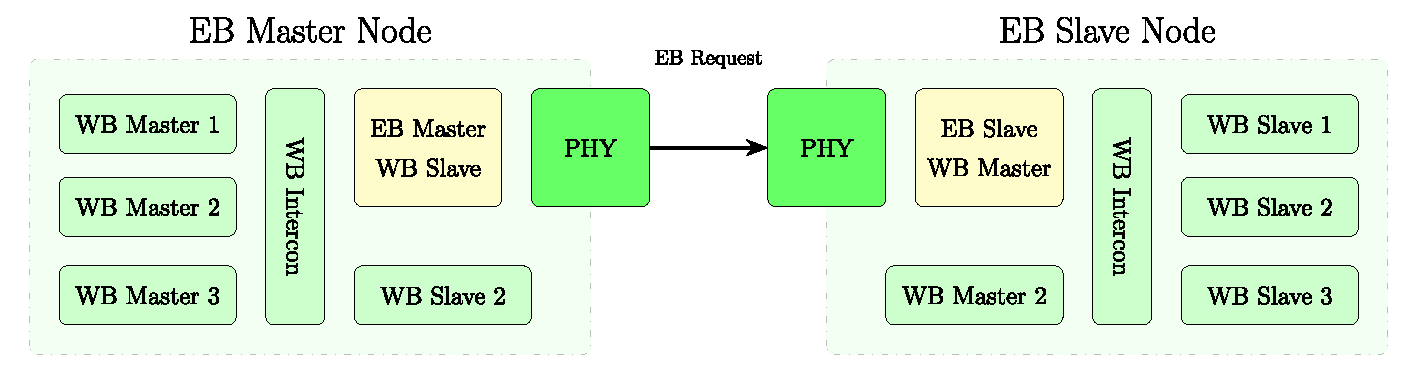
\includegraphics[width=15cm]{figures/EtherBone_1.pdf}
    \caption{EtherBone System}
    \label{fig:EtherBone-1}
\end{figure}

\vspace{5 mm}

\noindent Either or both of the devices may be replaced by software, as shown in figure \ref{fig:EtherBone-2}. 
In this scenario, the operating system buffers and sends Etherbone frames as requested by the Etherbone software library.
Client applications may use this library for remote access to any slave attached to an Etherbone equipped wishbone bus. 
This facilitates such tasks as debugging, firmware updates, and monitoring from a dekstop system. 
Applications may also attach devices to a virtual wishbone bus, perhaps to capture bus cycles or trigger an alarm. 
These virtual devices may be mapped into the Wishbone bus of other Etherbone nodes, hardware or software.

\begin{figure}[H]
    \centering
    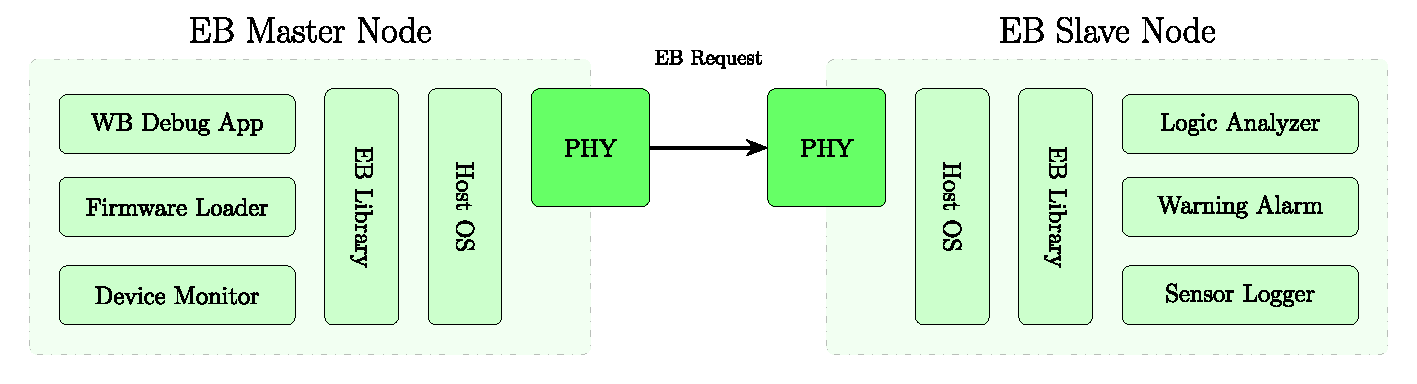
\includegraphics[width=15cm]{figures/EtherBone_2.pdf}
    \caption{EtherBone Software}
    \label{fig:EtherBone-2}
\end{figure}

\paragraph{Addressing}

Slaves on a Wishbone bus have a mapped address range. Masters read and write to an address on the local bus and the Intercon routes the operation to the matching slave device. 
However, with the introduction of Etherbone, there are now multiple reachable Wishbone buses in the facility-wide system. 
To select the destination slave, additional address information is required.

\vspace{5 mm}

\noindent When using the software interface, an application acquires a handle object for the remote bus. Reads and writes are then performed via the handle object, requiring only the WB bus address per operation. 
To acquire the handle object, the application supplies the hostname and port of the remote WB bus.

\vspace{5 mm}

\noindent For a hardware implementation, the requests come from a local WB master, which can only provide a WB bus address. 
To determine the missing address information, an EB bridge must infer the destination WB bus based only on the local WB address requested. 
To achieve this, the EB bridge establishes a configurable mapping from local WB addresses to destination hostname:ports and target WB addresses.

\vspace{5 mm}

\noindent For example, consider an EB bridge occupying address range \say{0x1000-0x3000} on the local bus. 
There is a remote WB bus available on the the host example.com:3434. 
We would like to access the address range \say{0x100-0x200} on that bus. Thus, we configure our EB bridge to map this range as \say{0x2000-0x2100} on the local bus. 
Now, when a WB write on our local bus to address \say{0x2050} is performed, the bridge transforms this into an EB write destined for example.com:3434 at address \say{0x150}.

\paragraph{Pipelining}
Unlike a local WB bus, where devices answer in a few clock cycles, a remote bus accessed via EB has a much high latency. 
For a 100MHz bus and a distance of only 20km the difference is 10ns to 100us. 
For Internet-scale distances, the latency can easily rise to 100ms.
Therefore, an application which only issues a new read/write operation when the previous operation completes will perform $10^4$ to $10^7$ times
slower over EB than direct WB.

\vspace{5 mm}

\noindent  EB supports pipelining to overcome this significant performance bottleneck. 
Instead of issuing a single operation at a time, an application/device can issue new operations without waiting for the previous operation to complete. 
The results of the operations will arrive in the same order they were issued. 
Whenever new operations do not dependend on still incomplete operations, this can almost entirely mask the performance lost to remote access.

\vspace{5 mm}

\noindent As an example, considering two application using EB. 
The first application is a firmware writing tool that needs to write the firmware and confirm the firmware was written correctly. 
This problem can be readily pipelined; the operations have an order requirement (confirmation happens after write), but the choice of operation to issue
does not depend on previous results. 
The firmware writer can issue a sequence of \say{WWWW...RRRR...} operations in the pipeline without waiting.
Alternatively, it might also use the sequence \say{WRWRWR...} to confirm each word immediately after writing it. 
In both cases, the application can issue all of the operations without waiting. 
This would not be possible if the application were to iterate a remote function. 
Suppose the application wants to compute \say{f(f(f(...f(x)...)))} using a remote WB slave to calculate function f. 
Here, the aplication writes x to the remote slave and reads back \say{y = f(x)}. 
Then the application writes y to the remote slave and reads back \say{z = f(y)}.
The write pattern \say{WRWRWR...} is the same as the firmware loader, but here we can only pipeline a single write-read operation pair together. 
Until we have received the result f(x), we cannot issue f(y).

\vspace{5 mm}

\noindent In Wishbone, several operations can be grouped into a single bus cycle.
A particularly bad situation that can occur is when dependencies appear within a WB cycle. 
Generally, WB cycles acquire the device for use until cycle completion. 
On a local bus, any access pattern will work, as the operations will complete quickly and release the cycle line. 
However, when this happens with EB-sized latencies, a cycle might tie up a device for potentially unacceptable duration. 
Consider for example a WB cycle that reads from one address and writes the result to another address.
Locally, there is no problem; the entire WB cycles executes in a few nanoseconds. 
However, when that same access pattern runs over the network, the slave device needs to wait for the read result to travel to the master and the final write to travel back. 
A very bad design.

\vspace{5 mm}

\noindent Dealing with data dependencies within a cycle is a major complication addressed in the different implementation options described later.

\paragraph{Config Space}

In addition to remote bus access, Etherbone also provides a configuration space. 
This config space is used to specify transmission parameters, recover bus error status codes, and match read results to the requests.

\vspace{5 mm}

\noindent The config space is an complementary 16-bit wide address space attached to every EB slave. 
EB requests can read/write to this configuration space in addition the the normal WB bus. 
The config space is divided up into two regions: the register space and the implementation space. 
All addresses in the register space correspond to EB control registers, specified in this document. 
The register space spans addresses \say{0x0-0x7FFF}. 
The implementation space is guaranteed to be free for whatever use a hardware/software implementation chooses. 
The implementation space spans \say{0x8000-0xFFFF}.

\vspace{5 mm}

\noindent Two important registers in the address space include the error status register, which reports WB error status codes, and the WB device map
pointer, which provides information about the slaves attached to a remote bus. 
The implementation space is typically used by an EB master to receive the data which it read. 
Reads to an EB device trigger a write back to the source EB device. 
Those writebacks are often sent to the implementation space where they can be handled by the EB core/code and invisible to the WB bus.

\paragraph{Bus Widths}

In Wishbone, a bus may have a port width that is \say{8/16/32/64} bits wide.
Thus, a master in one WB bus might write 32-bits at a time, while a slave in another WB bus expects 16-bits at a time. 
Etherbone makes no attempt to convert between differing port widths, because converting a 32-bit write into two 16-bit writes might change semantics.

\vspace{5 mm}

\noindent However, Etherbone does negotiate which port widths are acceptable to both devices. 
This mostly affects software, which can meaningfully support access with different port widths. 
Hardware implementations will typically advertise and accept only one width.

\vspace{5 mm}

\noindent Address spaces in WB are conceptually infinite, but in practice are constrained to a fixed width. 
Address width conversion, as oppposed to port width conversion, is relatively straight-forward. 
Address \say{0x0400} is that same as \say{0x00000400}. 
If a 32-bit device is accessed by a 16-bit device, the 16-bit device can only see the low 16-bits of the larger device's address space.

\vspace{5 mm}

\noindent Address width is negotiated by Etherbone simply to determine the amount of space to reserve for message exchanges. 
A hardware implementation is free to only advertise address widths whose message alignment is convenient to them.

\subsubsection{Chronos Project}

Chronos is an advanced timing and synchronization project at CERN, designed to support extremely precise timekeeping requirements in high-energy physics experiments. 

\vspace{5 mm}

\noindent Built on the foundations of the White Rabbit Project, Chronos \cite{gl:chronos} aims to improve upon CERN’s existing timing systems by achieving even more refined synchronization, essential for coordinating complex experiments and data acquisition across CERN’s infrastructure.

\subsection{SPAD Sensors}

SPAD (Single-Photon Avalanche Diode) \cite{9031298} sensors are an advanced type of photodiode sensor, specifically designed to detect extremely low amounts of light, to the single photon level. 
This makes them ideal for applications requiring exceptional sensitivity and the ability to measure extremely \textbf{fast} light events.

\vspace{5 mm}

\noindent Characteristics and Operation of SPADs:

\begin{itemize}
\item High Sensitivity
    \begin{itemize}
    \item[>] SPAD sensors can detect single photons, thanks to their ability to produce an \say{avalanche} of current when a single photon is detected.
    \item[>] This mechanism allows the sensor to significantly amplify the photon signal, providing a clear and strong response.
    \end{itemize}
\item Fast Response Time
    \begin{itemize}
    \item[>] SPADs are capable of recording events in times on the order of picoseconds.
    \item[>] This is useful in applications that require accurate photon arrival time (known as Time-of-Flight or TOF) measurements, such as in LIDAR and Time-Correlated Single Photon Counting (TCSPC), which is used in fluorescence studies.
    \end{itemize}
\item Geiger Mode Operation
    \begin{itemize}
    \item[>] SPADs operate in \say{Geiger} mode, which means that they are polarized at a voltage above the breakdown voltage. 
    \item[>] This causes an electron avalanche when a photon is detected, which allows the detection of the photon to be clearly recorded.
    \item[>] After detection, the sensor \textbf{needs a reset} to be ready for the next event.
    \end{itemize}
\item Dark noise/dark count noise
    \begin{itemize}
    \item[>] Although SPADs are very sensitive, they can suffer from “dark noise”, i.e. false signals caused by thermal electrons in the absence of light. 
    \item[>] This can be significantly controlled with cooling systems or by using signal processing techniques to filter out false events.
    \end{itemize}
\end{itemize}

\vspace{5 mm}

\noindent SPAD Sensor Applications:

\vspace{5 mm}

\noindent SPAD sensors are useful in many areas because of their their photon-level light detection capability and fast response.

\begin{itemize}
\item LIDAR (Light Detection and Ranging)
    \begin{itemize}
    \item[>] SPADs are an ideal choice for high-precision LIDAR systems that measure distances based on the time of flight of reflected photons. 
    \item[>] This is useful in autonomous vehicles, mapping, and environmental monitoring.
    \end{itemize}
\item Biomedicine and Microscopy
    \begin{itemize}
    \item[>] In fluorescence microscopy, SPADs are used for precise photon detection in molecular dynamics studies, where scientists analyze how molecules interact as a function of time.
    \end{itemize}
\item Time-of-Flight (ToF) cameras
    \begin{itemize}
    \item[>] These cameras, which are used in smartphones and augmented reality devices, employ SPAD sensors to capture \textbf{depth information}.
    \item[>] This allows measuring the distance to each point in the image, creating 3-D maps of the environment.
    \end{itemize}
\item Quantum Communications
    \begin{itemize}
    \item[>] SPADs are essential in quantum communications and quantum cryptography, as they can detect single photons that carry quantum information without loss of the signal integrity.
    \end{itemize}
\end{itemize}

\vspace{5 mm}

\noindent Advantages and Disadvantages

\begin{itemize}
\item Advantages:
    \begin{itemize}
    \item[>] Extreme photon sensitivity, appropriate for low light conditions.
    \item[>] Ultra-fast response time, ideal for precise detection and analysis applications.
    \item[>] Quantum information processing capability, important in cryptography and fundamental science.
    \end{itemize}
\item Disadvantages:
    \begin{itemize}
    \item[>] Dark noise, which can limit its accuracy if not properly controlled.
    \item[>] Cost and complexity of manufacture, making them more expensive than other conventional light sensors.
    \item[>] Need for cooling systems in applications where dark noise is critical, which can complicate system design.
    \end{itemize}
\end{itemize}

\subsection{TSN}

\subsection{RISC-V}

\subsection{Neuromorphic Sensors}

\newpage

\section{ASIC}

The goal of this thesis is to perform this ASIC:

\begin{figure}[H]
    \centering
    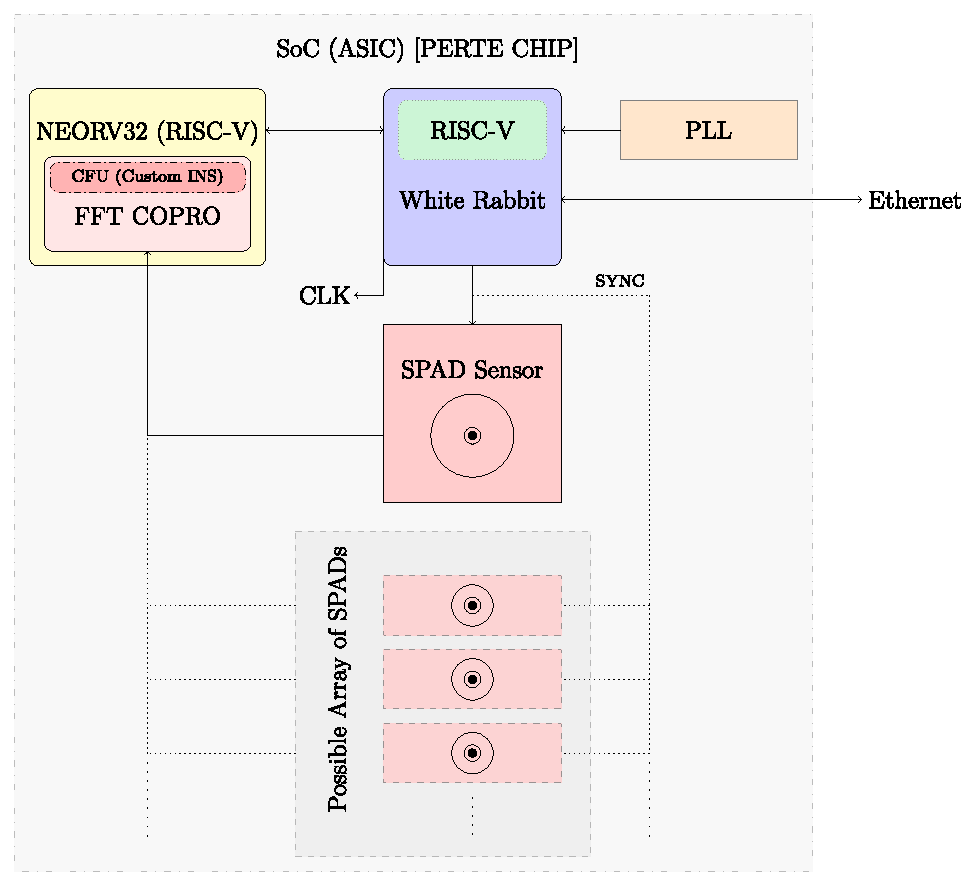
\includegraphics[width=14cm]{figures/ASIC-Scheme.pdf}
    \caption{ASIC to be develop.}
    \label{fig:ASIC}
\end{figure}

\newpage

\section{White Rabbit Node}

See White Rabbit Wiki \cite{WR:wiki}.

\begin{figure}[H]
    \centering
    \includegraphics[width=15cm]{figures/WR_node.pdf}
    \caption{WR Node.}
    \label{fig:WR-NODE}
\end{figure}

\newpage

\section{White Rabbit PTP Core}

The WR PTP (Precision Time Protocol) Core (WRPC) \cite{WR-core:wiki} \cite{WR-core:manual} \cite{WRPC:ohwr}, figure \ref{fig:WRPC}, is an Ethernet MAC implementation capable of providing precise timing. 
It can be used for sending and receiving regular Ethernet frames between user-defined HDL modules and a physical medium. 
It also implements the White Rabbit protocol to provide sub-nanosecond time synchronization.

\vspace{5 mm}

\noindent The White Rabbit PTP Core can operate in one of the following modes:
 
\begin{itemize}
\item GrandMaster:
    \begin{itemize}
    \item[>] WR Master synchronized to an external 1-PPS and 10 MHz clock signal, propagates precise timing to other WR-compliant devices.
    \end{itemize}
\item Master:
    \begin{itemize}
    \item[>] WR Master with free-running oscillator, propagates precise timing to other WR-compliant devices.
    \end{itemize}
\item Slave:
    \begin{itemize}
    \item[>] synchronizes its internal oscillator to another WR Master device.
    \end{itemize}
\end{itemize}

\begin{figure}[H]
    \centering
    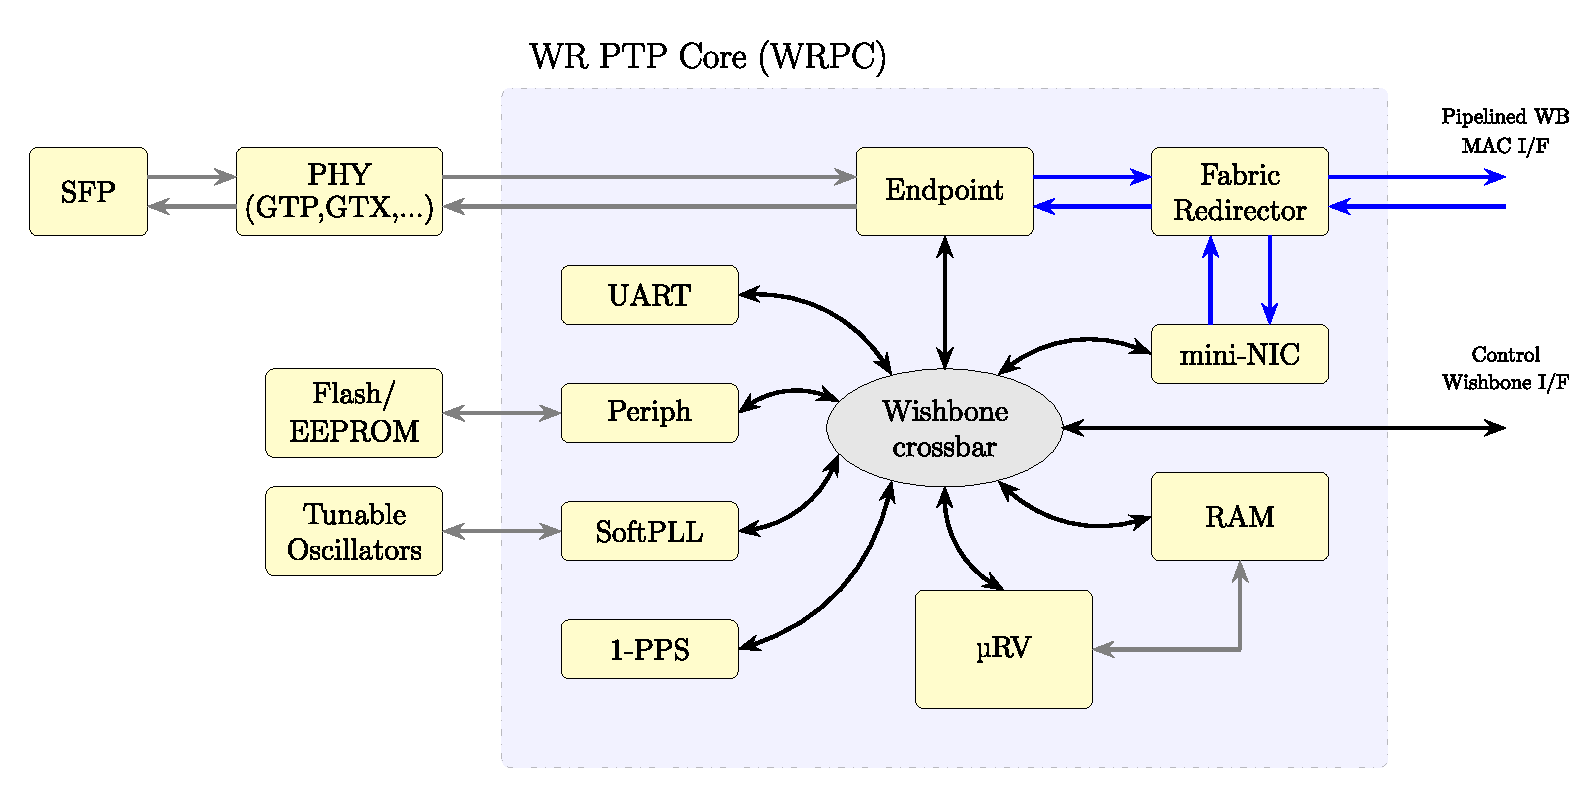
\includegraphics[width=15cm]{figures/WRPC.pdf}
    \caption{WR PTP (Precision Time Protocol) Core (WRPC).}
    \label{fig:WRPC}
\end{figure}

\noindent You can find the HDL description of the WRPC internal components in \cite{WRPC:modules}.

\newpage

\subsection{\textmu RV}

The \textmu RV \cite{urv-core:ohwr} \cite{urv-core:wiki} \cite{Włostowski:2213516} (Micro RISC-V) core is a small-sized implementation of a 32-bit RISC-V core, targeted specifically at FPGAs developed by CERN. 

\begin{figure}[H]
    \centering
    
\includegraphics[width=5cm]{figures/urv_logo.png}
    \caption{\textmu RV logo.}
    \label{fig:urv}
\end{figure}

\begin{itemize}
\item Features:
    \begin{itemize}
    \item[>] Supports RV32IM instruction set. 
Division and multiply high instructions are optional and can be emulated to lower the FPGA footprint.
    \item[>] Target: FPGAs.
    \item[>] 4-stage pipeline (FDXW).
    \item[>] All instructions except taken branches/division in one clock cycle.
    \item[>] Code execution from internal memory block.
    \item[>] Wishbone bus (version B.4) for peripheral access.
    \item[>] Simple interrupt handling.
    \item[>] Verilog RTL code.
    \end{itemize}
\end{itemize}

\noindent Since \textmu RV is described in verilog and most of the WRPC component is in VHDL, it will be necessary to use a \textbf{mixed simulator} supported by VUnit.
In this context, one of the best options is \say{QuestaSim}.

\vspace{5mm}

\noindent \href{https://github.com/umarcor}{Umarcor} is planning to develop a container, hosted on our server, for this purpose. 
(DONE - Questa container, with and without VUnit, available on the lab server.)

\vspace{5mm}

\noindent \textbf{Task:} Learn how to generate a testbench using both HDLs: VHDL and Verilog.
(Initial mixed simulation test DONE - Unfortunately questa is a proprietary software and our server image cannot be distributed, so this example cannot be shown on GitHub, it is only available in our private GitLab repository.)

\newpage
\section{White Rabbit Node}
\label{wrn}

See White Rabbit Wiki \cite{WR:wiki}.

\begin{figure}[H]
    \centering
    \includegraphics[width=15cm]{figures/WR_node.pdf}
    \caption{WR Node.}
    \label{fig:WR-NODE}
\end{figure}

\newpage
\section{White Rabbit PTP Core}

The WR PTP (Precision Time Protocol) Core (WRPC) \cite{WR-core:wiki} \cite{WR-core:manual} \cite{WRPC:ohwr}, figure \ref{fig:WRPC}, is an Ethernet MAC implementation capable of providing precise timing. 
It can be used for sending and receiving regular Ethernet frames between user-defined HDL modules and a physical medium. 
It also implements the White Rabbit protocol to provide sub-nanosecond time synchronization.

\vspace{5 mm}

\noindent The White Rabbit PTP Core can operate in one of the following modes:
 
\begin{itemize}
\item GrandMaster:
    \begin{itemize}
    \item[>] WR Master synchronized to an external 1-PPS and 10 MHz clock signal, propagates precise timing to other WR-compliant devices.
    \end{itemize}
\item Master:
    \begin{itemize}
    \item[>] WR Master with free-running oscillator, propagates precise timing to other WR-compliant devices.
    \end{itemize}
\item Slave:
    \begin{itemize}
    \item[>] synchronizes its internal oscillator to another WR Master device.
    \end{itemize}
\end{itemize}

\begin{figure}[H]
    \centering
    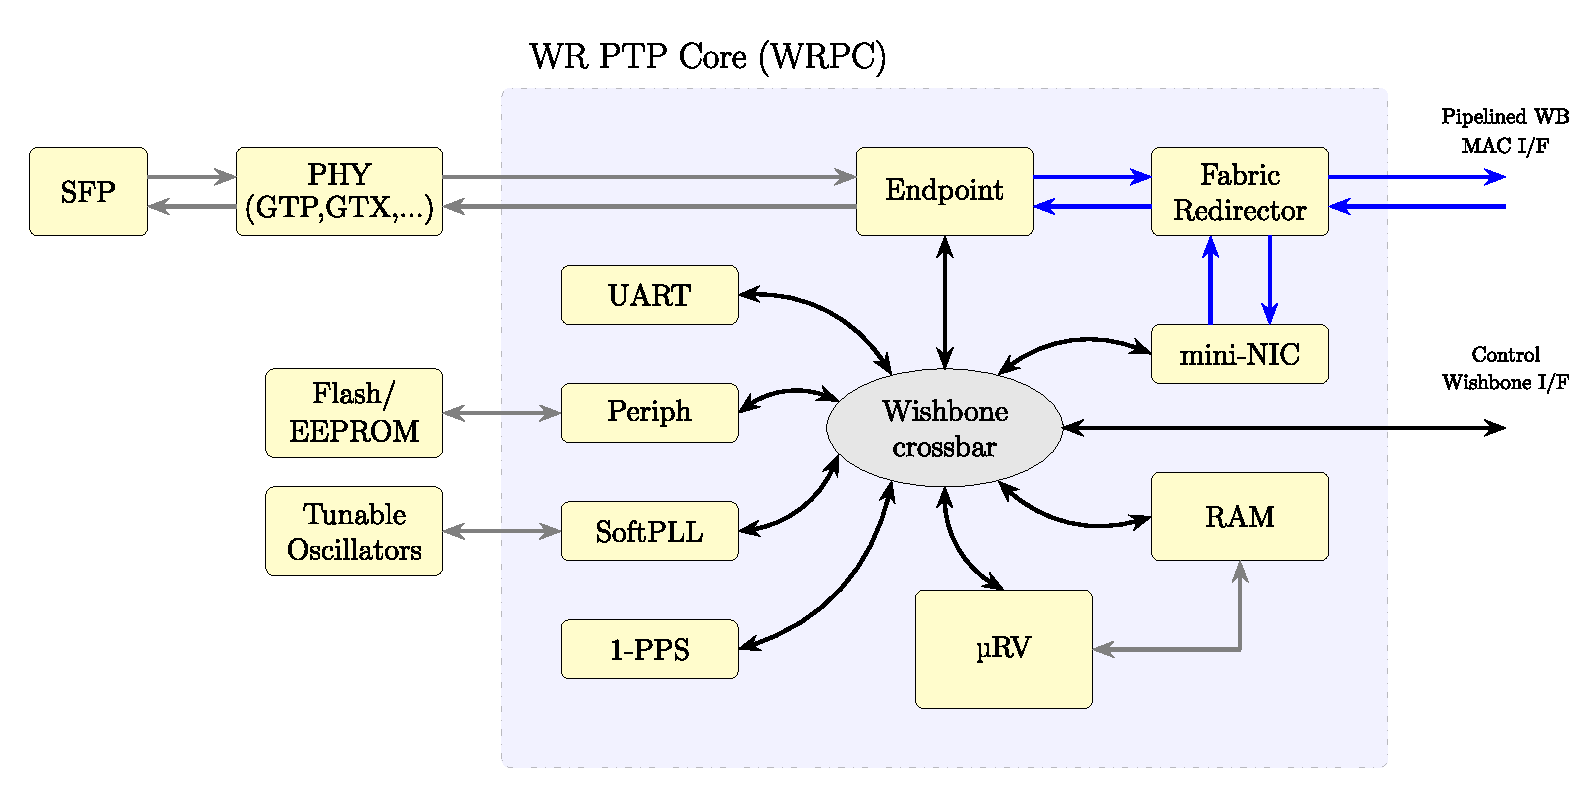
\includegraphics[width=15cm]{figures/WRPC.pdf}
    \caption{WR PTP (Precision Time Protocol) Core (WRPC).}
    \label{fig:WRPC}
\end{figure}

\noindent You can find the HDL description of the WRPC internal components in \cite{WRPC:modules}.

\subsection{\textmu RV}

The \textmu RV \cite{urv-core:ohwr} \cite{urv-core:wiki} \cite{Włostowski:2213516} (Micro RISC-V) core is a small-sized implementation of a 32-bit RISC-V core, targeted specifically at FPGAs developed by CERN. 

\begin{figure}[H]
    \centering
    
\includegraphics[width=5cm]{figures/urv_logo.png}
    \caption{\textmu RV logo.}
    \label{fig:urv}
\end{figure}

\begin{itemize}
\item Features:
    \begin{itemize}
    \item[>] Supports RV32IM instruction set. 
Division and multiply high instructions are optional and can be emulated to lower the FPGA footprint.
    \item[>] Target: FPGAs.
    \item[>] 4-stage pipeline (FDXW).
    \item[>] All instructions except taken branches/division in one clock cycle.
    \item[>] Code execution from internal memory block.
    \item[>] Wishbone bus (version B.4) for peripheral access.
    \item[>] Simple interrupt handling.
    \item[>] Verilog RTL code.
    \end{itemize}
\end{itemize}

\noindent Since \textmu RV is described in verilog and most of the WRPC component is in VHDL, it will be necessary to use a \textbf{mixed simulator} supported by VUnit.
In this context, one of the best options is \say{QuestaSim}.

\vspace{5mm}

\noindent \href{https://github.com/umarcor}{Umarcor} is planning to develop a container, hosted on our server, for this purpose. 
(DONE - Questa container, with and without VUnit, available on the lab server.)

\vspace{5mm}

\noindent \textbf{Task:} Learn how to generate a testbench using both HDLs: VHDL and Verilog.
(Initial mixed simulation test DONE - Unfortunately questa is a proprietary software and our server image cannot be distributed, so this example cannot be shown on GitHub, it is only available in our private GitLab repository.)

\subsection{WRPC Simulation}

\subsubsection{WRPC v4.2 for Spartan6 - LM32}
\label{list-wrpc}

I've successfully simulated WRPC \cite{WRPC:ohwr} in its \say{v4.2} version for \textbf{Spartan6} FPGA.

\vspace{5mm}

\noindent See \href{https://github.com/Unike267/Thesis/issues/2}{github.com/Unike267/Thesis/issues/2} to check how I have done it.

\vspace{5mm}

\noindent HDL modules that form the WRPC (\say{v4.2} for Spartan6) are:

\newpage 

\begin{dig}
\item ip\_cores
    \begin{dig}
    \item etherbone-core
        \begin{dig}
        \item hdl
            \begin{dig}
            \item eb\_master\_core (VHDL)
            \item eb\_slave\_core (VHDL)
            \item eb\_usb\_core (VHDL)
            \end{dig}
        \end{dig}
    \item general-cores
        \begin{dig}
        \item modules
            \begin{dig}
            \item common (VHDL)
            \item genrams
                \begin{dig}
                \item . (VHDL)
                \item common (VHDL)
                \item generic (VHDL)
                \item xilinx (VHDL)
                \end{dig}
            \item wishbone
                \begin{dig}
                \item . (VHDL)
                \item wb\_async\_bridge (VHDL)
                \item wb\_axi4lite\_bridge (VHDL)
                \item wb\_bus\_fanout (VHDL)
                \item wb\_clock\_crossing (VHDL)
                \item wb\_crossbar (VHDL)
                \item wb\_dma (VHDL)
                \item wb\_dpram (VHDL)
                \item wb\_gpio\_port (VHDL)
                \item wb\_i2c\_bridge (VHDL)
                \item wb\_i2c\_master (VHDL)
                \item wb\_irq (VHDL)
                \item wb\_lm32
                    \begin{dig}
                    \item generated (Verilog and VHDL)
                    \item platform/spartan6 (Verilog)
                    \item src (Verilog and VHDL)
                    \end{dig}
                \item wb\_onewire\_master (Verilog and VHDL)
                \item wb\_serial\_lcd (VHDL)
                \item wb\_simple\_pwm (VHDL)
                \item wb\_simple\_timer (VHDL)
                \item wb\_slave\_adapter (VHDL)
                \item wb\_spi (Verilog and VHDL)
                \item wb\_spi\_flash (VHDL)
                \item wb\_uart (VHDL)
                \item wb\_vic (VHDL)
                \item wbgen2 (VHDL)
                \item wbgenplus (VHDL)
                \end{dig}
            \end{dig}
        \item platform/xilinx
            \begin{dig}
            \item wb\_xil\_multiboot (VHDL)
            \item wb\_xilinx\_fpga\_loader (VHDL)
            \end{dig}
        \end{dig}
    \item gn4124-core
        \begin{dig}
        \item hdl
        \begin{dig}
            \item gn4124core   
                \begin{dig}
                \item rtl
                    \begin{dig}
                    \item . (VHDL)
                    \item spartan6 (VHDL)
                    \end{dig}  
                \end{dig}            
            \item spec
                \begin{dig}
                \item ip\_cores (VHDL)
                \end{dig}  
            \end{dig}
        \end{dig}
    \end{dig}
\item modules
    \begin{dig}
    \item fabric
        \begin{dig}
        \item . (VHDL)
        \item xwrf\_loopback (VHDL)
        \end{dig}
    \item timing (VHDL)
    \item wr\_dacs (VHDL)
    \item wr\_eca (VHDL)
    \item wr\_endpoint (VHDL)
    \item wr\_mini\_nic (VHDL)
    \item wr\_pps\_gen (VHDL)
    \item wr\_si57x\_interface (VHDL)
    \item wr\_softpll\_ng (VHDL)
    \item wr\_streamers (VHDL)
    \item wr\_tbi\_phy (VHDL)
    \item wr\_tlu (VHDL)
    \item wrc\_core (VHDL)
    \end{dig}
\item platform
    \begin{dig}
    \item xilinx
        \begin{dig}
        \item . (VHDL)
        \item wr\_gtp\_phy
            \begin{dig}
            \item . (VHDL)
            \item spartan6 (VHDL)
            \end{dig}
        \end{dig}
    \end{dig}
\end{dig}

\newpage 

\noindent HDL files for simulation are:

\begin{dig}
\item sim
    \begin{dig}
    \item endpoint\_mdio.v
    \item endpoint\_regs.v
    \item eth\_packet.svh
    \item if\_wb\_link.svh
    \item if\_wb\_master.svh
    \item if\_wb\_slave.svh
    \item if\_wishbone\_accessor.svh
    \item if\_wishbone\_types.svh
    \item lbk\_regs.v
    \item minic\_regs.vh
    \item simdrv\_defs.svh
    \item tbi\_utils.sv
    \item wb\_fabric\_defs.svh
    \item wb\_packet\_sink.svh
    \item wb\_packet\_source.svh
    \item wrc\_syscon\_regs.vh
    \item drivers:
        \begin{dig}
        \item simdrv\_minic.svh
        \item simdrv\_wr\_endpoint.svh 
        \end{dig}
    \end{dig}
\item testbench
    \begin{dig}
    \item wrc\_core
        \begin{dig}
        \item main.sv 
        \item functions.svh 
        \end{dig}
    \end{dig}
\end{dig}

\vspace{5mm}

\noindent According to this list of modules, I've generated the following block diagram shown in \ref{fig:dig}.

\vspace{5mm}

\noindent The green zone of the figure corresponds to the modules located in the \say{ip\_core} directory, the red zone to those in \say{modules}, and the blue zone to those in \say{platform}.

\begin{landscape}
\newgeometry{
	paper=a4paper, % Change to letterpaper for US letter
	inner=1cm, % Inner margin
	outer=4cm, % Outer margin
	bindingoffset=.5cm, % Binding offset
	top=12cm, % Top margin
	bottom=-5cm, % Bottom margin
	%showframe, % Uncomment to show how the type block is set on the page
}

\begin{figure}[H]
    \centering
    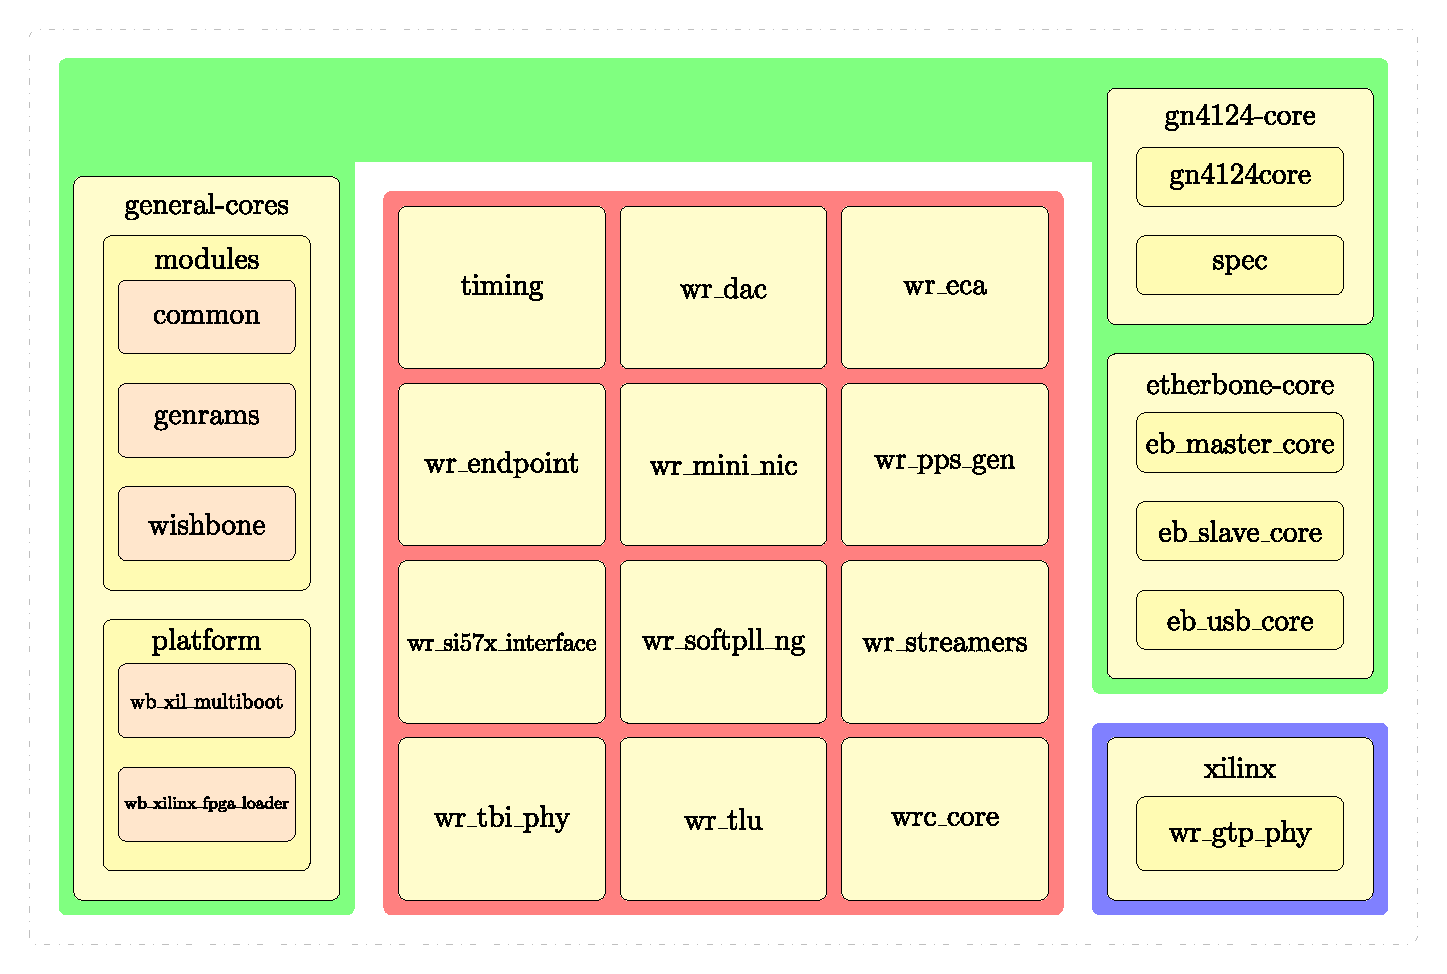
\includegraphics[width=26cm]{figures/wrpc-sources-diagram.pdf}
    \captionsetup{name=\hspace{8.5cm}Figure,format=plain,justification=centering,width=20cm}
    \caption{Block diagram of WRPC v4.2 sources for Spartan6.}
    \label{fig:dig}
\end{figure}
\restoregeometry
\end{landscape}

\noindent Taking a closer look at the \say{main.sv} testbench, I summarized the inputs and outputs of the four different modules imported into the test, which are:

\begin{itemize}
\item Clock/reset generator
\item Design Under Test: WRPC
\item Endpoint
\item Loopback
\end{itemize}

\noindent The following list presents them:

\begin{dig}
\item tbi\_clock\_rst\_gen/clkgen:
    \begin{dig}
    \item OUTPUTS:
        \begin{dig}
        \item .clk\_ref\_o                    (clk\_ref)
        \item .clk\_sys\_o                    (clk\_sys)
        \item .phy\_rbclk\_o                  (phy\_rbclk)
        \item .rst\_n\_o                      (rst\_n)
        \end{dig}
    \end{dig}
\item wr\_core/DUT (WR PTP CORE):
    \begin{dig}
    \item INPUTS:
        \begin{dig}
        \item .clk\_sys\_i                    (clk\_sys)
        \item .clk\_dmtd\_i                   (clk\_ref)
        \item .clk\_ref\_i                    (clk\_ref)
        \item .rst\_n\_i                      (rst\_n)
        \item UART:
            \begin{dig}
            \item .uart\_rxd\_i                   (1'b0)
            \end{dig}
        \item I2C:
            \begin{dig}
            \item .scl\_i                      (scl\_loop)
            \item .sda\_i                      (sda\_loop)
            \end{dig}
        \item .btn1\_i                     (1'b0)
        \item .btn2\_i                     (1'b0)
        \item Connected to wrf\_loopback:
            \begin{dig}
            \item .ext\_snk\_adr\_i              (wrc\_snk\_adr)
            \item .ext\_snk\_dat\_i              (wrc\_snk\_dat)
            \item .ext\_snk\_sel\_i              (wrc\_snk\_sel)
            \item .ext\_snk\_cyc\_i              (wrc\_snk\_cyc)
            \item .ext\_snk\_we\_i               (1'b1)
            \item .ext\_snk\_stb\_i              (wrc\_snk\_stb)
            \item 
            \item .ext\_src\_ack\_i              (wrc\_src\_ack)
            \item .ext\_src\_err\_i              (wrc\_src\_err)
            \item .ext\_src\_stall\_i            (wrc\_src\_stall)
            \end{dig}
        \item WISHBONE:
            \begin{dig}
            \item .wb\_adr\_i                   (WB\_wrc.master.adr[31:0])
            \item .wb\_dat\_i                   (WB\_wrc.master.dat\_o)
            \item .wb\_sel\_i                   (4'b1111)
            \item .wb\_we\_i                    (WB\_wrc.master.we)
            \item .wb\_cyc\_i                   (WB\_wrc.master.cyc)
            \item .wb\_stb\_i                   (WB\_wrc.master.stb)
            \end{dig}
        \item PHY:
            \begin{dig}
            \item .phy\_ref\_clk\_i              (clk\_ref)
            \item .phy\_tx\_disparity\_i         (phy\_tx\_disparity)
            \item .phy\_tx\_enc\_err\_i           (phy\_tx\_enc\_err)
            \item .phy\_rx\_rbclk\_i             (clk\_ref)
            \item .phy\_rx\_data\_i              (phy\_rx\_data)
            \item .phy\_rx\_k\_i                 (phy\_rx\_k)
            \item .phy\_rx\_enc\_err\_i           (phy\_rx\_enc\_err)
            \item .phy\_rx\_bitslide\_i          (phy\_rx\_bitslide)
            \end{dig}
        \end{dig}
    \item OUTPUTS:
        \begin{dig}
        \item .pps\_p\_o                    ()
        \item .dac\_hpll\_load\_p1\_o         ()
        \item .dac\_hpll\_data\_o            ()
        \item .dac\_dpll\_load\_p1\_o         ()
        \item .dac\_dpll\_data\_o            ()
        \item UART:
            \begin{dig}
            \item .uart\_txd\_o                 ()
            \end{dig}
        \item I2C:
            \begin{dig}
            \item .scl\_o                      (scl\_loop)
            \item .sda\_o                      (sda\_loop)
            \end{dig}
        \item .led\_link\_o                 (link\_up)
        \item connected to wrf\_loopback
            \begin{dig}
            \item .ext\_snk\_ack\_o              (wrc\_snk\_ack)
            \item .ext\_snk\_err\_o              (wrc\_snk\_err)
            \item .ext\_snk\_stall\_o            (wrc\_snk\_stall)
            \item 
            \item .ext\_src\_adr\_o              (wrc\_src\_adr)
            \item .ext\_src\_dat\_o              (wrc\_src\_dat)
            \item .ext\_src\_sel\_o              (wrc\_src\_sel)
            \item .ext\_src\_cyc\_o              (wrc\_src\_cyc)
            \item .ext\_src\_stb\_o              (wrc\_src\_stb)
            \item .ext\_src\_we\_o               ()
            \end{dig}
        \item WISHBONE:
            \begin{dig}
            \item .wb\_dat\_o                   (WB\_wrc.master.dat\_i)
            \item .wb\_ack\_o                   (WB\_wrc.master.ack)
            \item .wb\_stall\_o                 (WB\_wrc.master.stall)
            \end{dig}
        \item PHY:
            \begin{dig}
            \item .phy\_tx\_data\_o              (phy\_tx\_data)
            \item .phy\_tx\_k\_o                 (phy\_tx\_k)
            \item .phy\_rst\_o                  (phy\_rst)
            \item .phy\_loopen\_o               (phy\_lo)
            \end{dig}
        \end{dig}
    \end{dig}
\item wr\_endpoint/EP (ENDPOINT):
    \begin{dig}
    \item INPUTS:
        \begin{dig}
        \item .clk\_ref\_i                  (clk\_ref)
        \item .clk\_sys\_i                  (clk\_sys)
        \item .clk\_dmtd\_i                 (clk\_ref)
        \item .rst\_sys\_n\_i                (rst\_n)
        \item .rst\_ref\_n\_i                (rst\_n)
        \item .rst\_dmtd\_n\_i               (rst\_n)
        \item .rst\_txclk\_n\_i              (rst\_n)
        \item .rst\_rxclk\_n\_i              (rst\_n)
        \item .pps\_csync\_p1\_i             (1'b0)
        \item PHY:
            \begin{dig}
            \item .phy\_sfp\_tx\_fault\_i         (1'b0)
            \item .phy\_sfp\_los\_i              (1'b0)
            \item .phy\_rdy\_i                  (1'b1)
            \item .phy\_ref\_clk\_i              (clk\_ref)
            \item .phy\_tx\_disparity\_i         (phy\_tx\_disparity)
            \item .phy\_tx\_enc\_err\_i           (phy\_tx\_enc\_err)
            \item .phy\_rx\_data\_i              (phy\_tx\_data)
            \item .phy\_rx\_clk\_i               (clk\_ref)
            \item .phy\_rx\_k\_i                 (phy\_tx\_k)
            \item .phy\_rx\_enc\_err\_i           (phy\_rx\_enc\_err)
            \item .phy\_rx\_bitslide\_i          (phy\_rx\_bitslide)
            \end{dig}
        \item Connected to simulation:
            \begin{dig}
            \item .src\_stall\_i                (WB\_ep\_snk.slave.stall)
            \item .src\_ack\_i                  (WB\_ep\_snk.slave.ack)
            \item .src\_err\_i                  (1'b0)
            \item 
            \item .snk\_dat\_i                  (WB\_ep\_src.master.dat\_o)
            \item .snk\_adr\_i                  (WB\_ep\_src.master.adr)
            \item .snk\_sel\_i                  (WB\_ep\_src.master.sel)
            \item .snk\_cyc\_i                  (WB\_ep\_src.master.cyc)
            \item .snk\_stb\_i                  (WB\_ep\_src.master.stb)
            \item .snk\_we\_i                   (WB\_ep\_src.master.we)
            \end{dig}
        \item WISHBONE:
            \begin{dig}
            \item .wb\_cyc\_i                   (WB\_ep.master.cyc)
            \item .wb\_stb\_i                   (WB\_ep.master.stb)
            \item .wb\_we\_i                    (WB\_ep.master.we)
            \item .wb\_sel\_i                   (WB\_ep.master.sel)
            \item .wb\_adr\_i                   (WB\_ep.master.adr[7:0])
            \item .wb\_dat\_i                   (WB\_ep.master.dat\_o)
            \end{dig}
        \end{dig}
    \item OUTPUTS:
        \begin{dig}
        \item PHY:
            \begin{dig}
            \item .phy\_tx\_data\_o              (phy\_rx\_data)
            \item .phy\_tx\_k\_o                 (phy\_rx\_k)
            \end{dig}
        \item Connected to simulation:
            \begin{dig}
            \item .src\_dat\_o                  (WB\_ep\_snk.slave.dat\_i)
            \item .src\_adr\_o                  (WB\_ep\_snk.slave.adr)
            \item .src\_sel\_o                  (WB\_ep\_snk.slave.sel)
            \item .src\_cyc\_o                  (WB\_ep\_snk.slave.cyc)
            \item .src\_stb\_o                  (WB\_ep\_snk.slave.stb)
            \item .src\_we\_o                   (WB\_ep\_snk.slave.we)
            \item 
            \item .snk\_stall\_o                (WB\_ep\_src.master.stall)
            \item .snk\_ack\_o                  (WB\_ep\_src.master.ack)
            \item .snk\_err\_o                  (WB\_ep\_src.master.err)
            \end{dig}
        \item WISHBONE:
            \begin{dig}
            \item .wb\_dat\_o                   (WB\_ep.master.dat\_i)
            \item .wb\_ack\_o                   (WB\_ep.master.ack)
            \item .wb\_stall\_o                 (WB\_ep.master.stall));
            \end{dig}
        \end{dig}
    \end{dig}
\item wrf\_loopback/WRF\_LBK (LOOPBACK): 
    \begin{dig}
    \item INPUTS:
        \begin{dig}
        \item .clk\_sys\_i                  (clk\_sys)
        \item .rst\_n\_i                    (rst\_n)
        \item Connected to wr\_core:
            \begin{dig}
            \item .snk\_cyc\_i                  (wrc\_src\_cyc)
            \item .snk\_stb\_i                  (wrc\_src\_stb)
            \item .snk\_we\_i                   (1'b1)
            \item .snk\_sel\_i                  (wrc\_src\_sel)
            \item .snk\_adr\_i                  (wrc\_src\_adr)
            \item .snk\_dat\_i                  (wrc\_src\_dat)
            \item 
            \item .src\_ack\_i                  (wrc\_snk\_ack)
            \item .src\_stall\_i                (wrc\_snk\_stall)
            \end{dig}
        \item WISHBONE:
            \begin{dig}
            \item .wb\_cyc\_i                   (WB\_lbk.master.cyc)
            \item .wb\_stb\_i                   (WB\_lbk.master.stb)
            \item .wb\_we\_i                    (WB\_lbk.master.we)
            \item .wb\_sel\_i                   (4'b1111)
            \item .wb\_adr\_i                   (WB\_lbk.master.adr)
            \item .wb\_dat\_i                   (WB\_lbk.master.dat\_o)
            \end{dig}
        \end{dig}
    \item OUTPUTS:
        \begin{dig}
        \item Connected to wr\_core:
            \begin{dig}
            \item .snk\_ack\_o                  (wrc\_src\_ack)
            \item .snk\_stall\_o                (wrc\_src\_stall)
            \item 
            \item .src\_cyc\_o                  (wrc\_snk\_cyc)
            \item .src\_stb\_o                  (wrc\_snk\_stb)
            \item .src\_we\_o                   ()
            \item .src\_sel\_o                  (wrc\_snk\_sel)
            \item .src\_adr\_o                  (wrc\_snk\_adr)
            \item .src\_dat\_o                  (wrc\_snk\_dat)
            \end{dig}
        \item WISHBONE:
            \begin{dig}
            \item .wb\_dat\_o                   (WB\_lbk.master.dat\_i)
            \item .wb\_ack\_o                   (WB\_lbk.master.ack)
            \end{dig}
        \end{dig}
    \end{dig}
\end{dig}

\newpage 

\noindent This simulation has been successfully integrated into the continuous integration pipeline of the GitLab repository, see \href{https://github.com/Unike267/Thesis/issues/3}{github.com/Unike267/Thesis/ issues/3}.
Some of the most important steps that have been carried out are:

\begin{dig}
\item Compile the necessary Xilinx libraries (\say{unisim} and \say{xilinxcorelib}) using ISE as an intermediary.
\item Generate the required Makefile using the hdlmake tool \cite{hdl-make:ohwr}.
\item Run the simulation with Questasim.
\item Upload the waveform as an artifact.
\end{dig}

\vspace{1mm}

\noindent This process is illustrated graphically through the following images:

\begin{figure}[H]
\centering
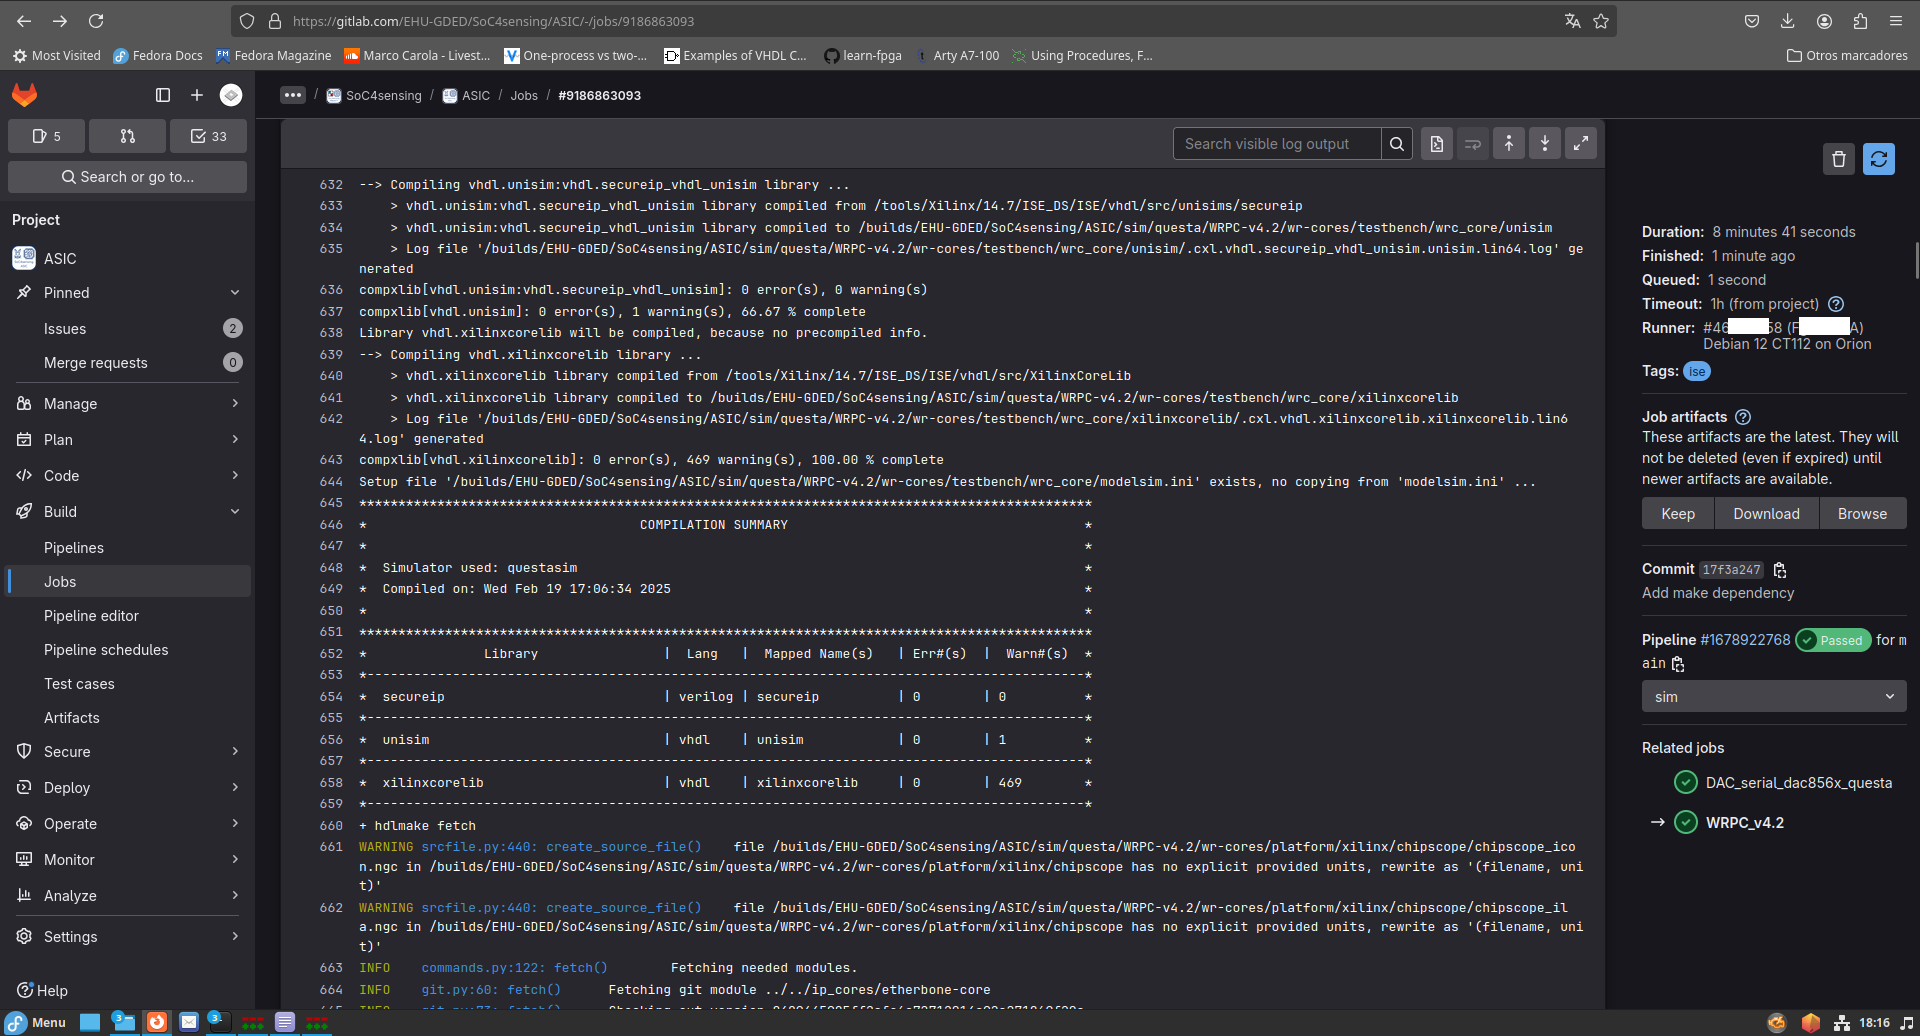
\includegraphics[width=14cm]{figures/wrpc_ci_1.png}
\caption{Compiling the Xilinx libraries and generating the Makefile.}
\label{fig:wrpc-ci-1}
\end{figure}

\begin{figure}[H]
\centering
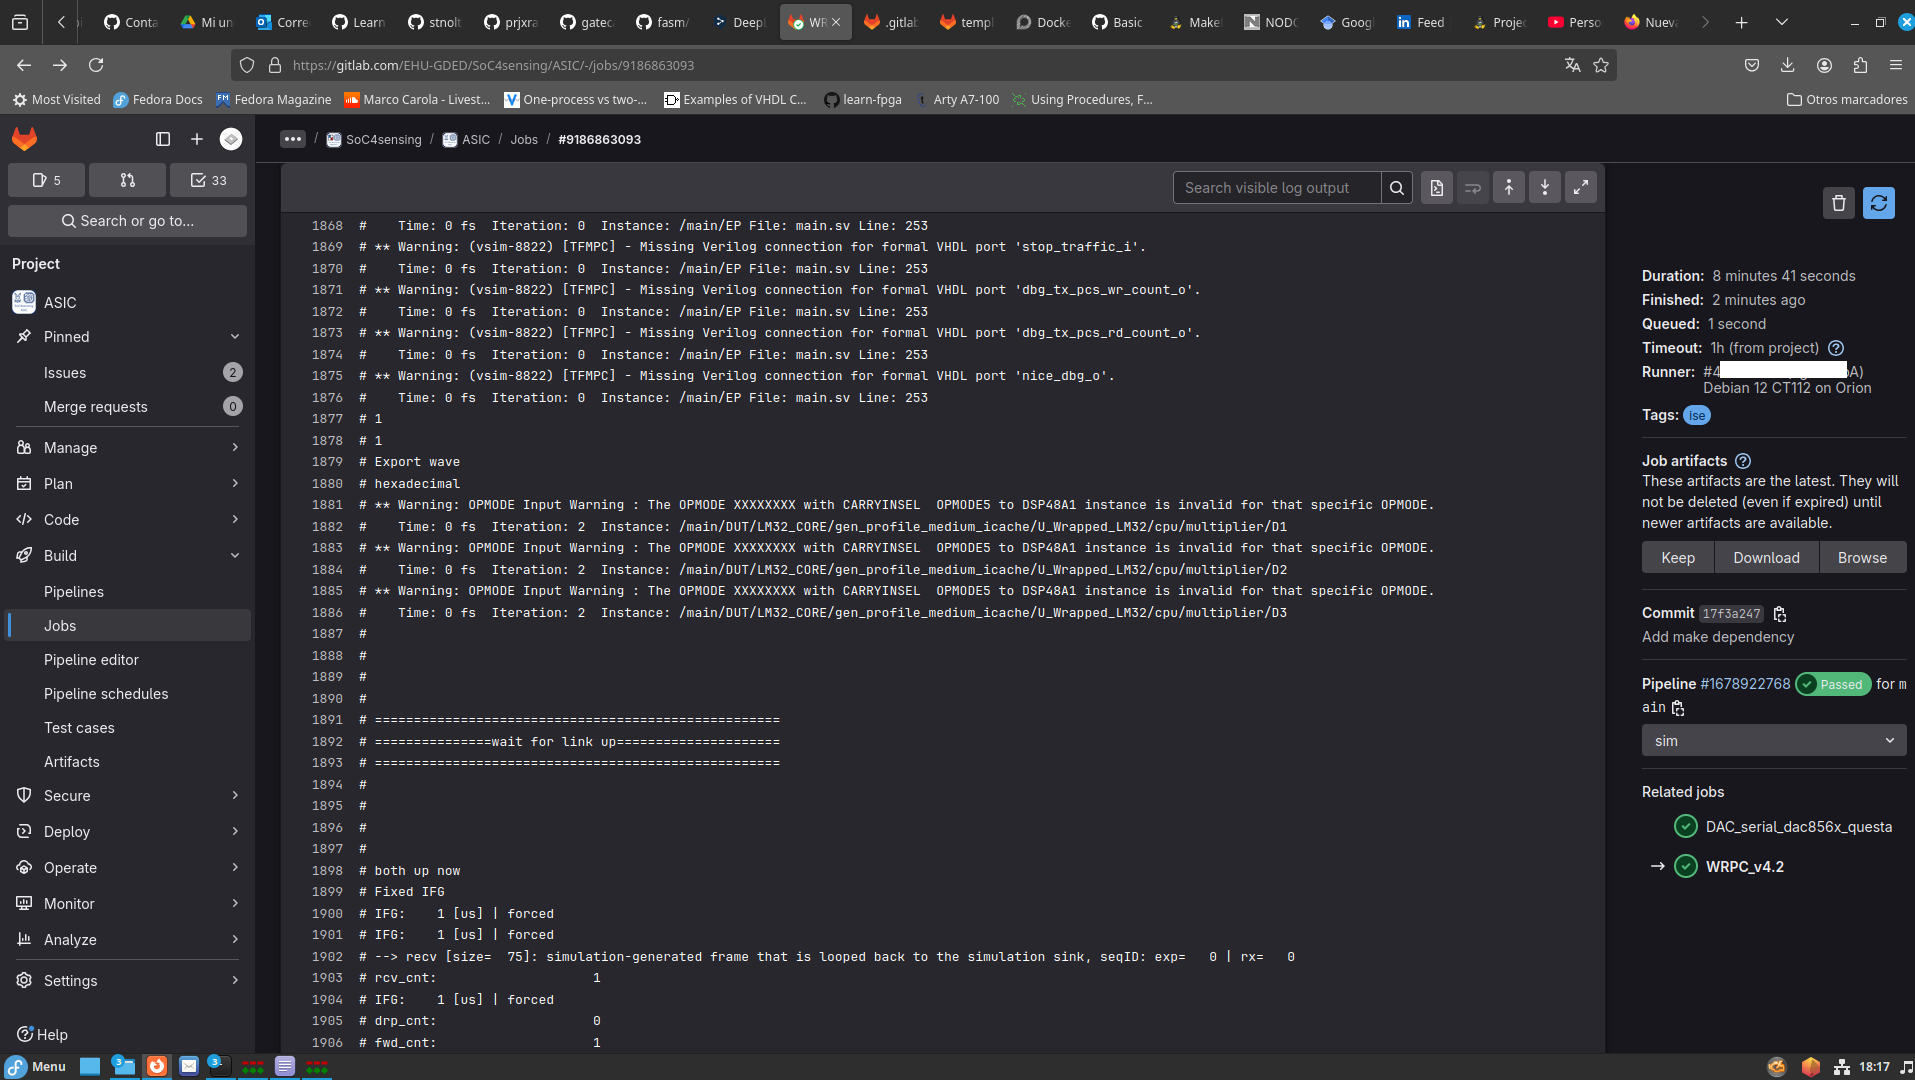
\includegraphics[width=14cm]{figures/wrpc_ci_2.png}
\caption{Running the simulation with Questasim.}
\label{fig:wrpc-ci-2}
\end{figure}

\begin{figure}[H]
\centering
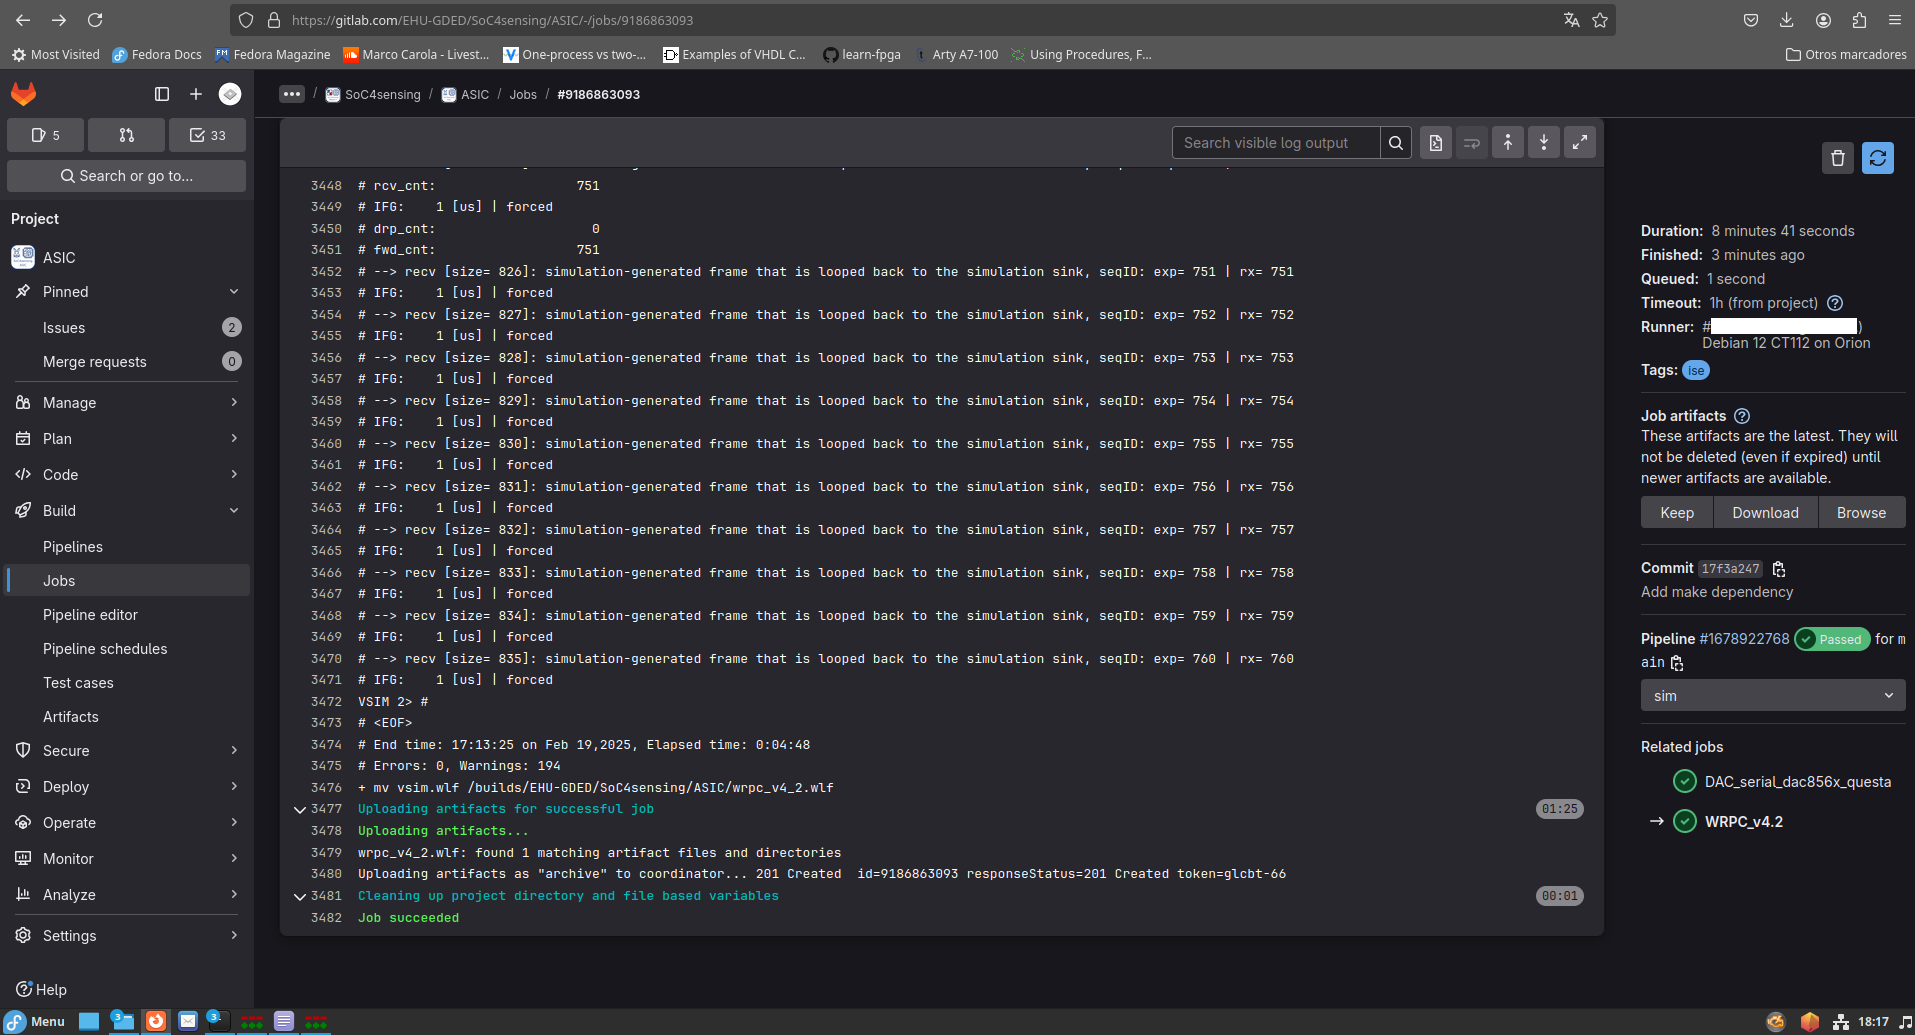
\includegraphics[width=14cm]{figures/wrpc_ci_3.png}
\caption{Uploading the waveform as an artifact.}
\label{fig:wrpc-ci-3}
\end{figure}

\subsubsection{DAC: serial\_dac856x}

\noindent As a proof of concept for performing simulation in continuous integration using free/libre tools, the \say{serial\_dac856x} DAC has been simulated.

\vspace{5mm}

\noindent This simulation was carried out using the VUnit \cite{gh:vunit} framework and the GHDL \cite{gh:ghdl} simulator.

\vspace{5mm}

\noindent Since there is no free/libre mixed-language simulator available, generating a complete WRPC simulation is not possible in the GitHub-hosted repository. However, this limitation does not apply to the GitLab repository, where we have access to a private container with Questasim and VUnit.

\vspace{5mm}

\noindent This restriction exists because several WRPC module sources are written in Verilog, see \ref{list-wrpc}.

\vspace{5mm}

\noindent The simulation results, including both the waveform and the \say{CSV} file containing the verbose output, are uploaded as artifacts and attached to the release assets, see \href{https://github.com/Unike267/Thesis/releases}{github.com/Unike267/Thesis/releases}.

\newpage
\section{ASIC}
\label{asic}

\st{The goal of this thesis is to perform this ASIC:}

\noindent The goal of the thesis is to perform an ASIC but this diagram doesn't show the real design at all.
Actually, the layout is currently being designed and when we have a valid result we will update the correct diagram.

\begin{figure}[H]
    \centering
    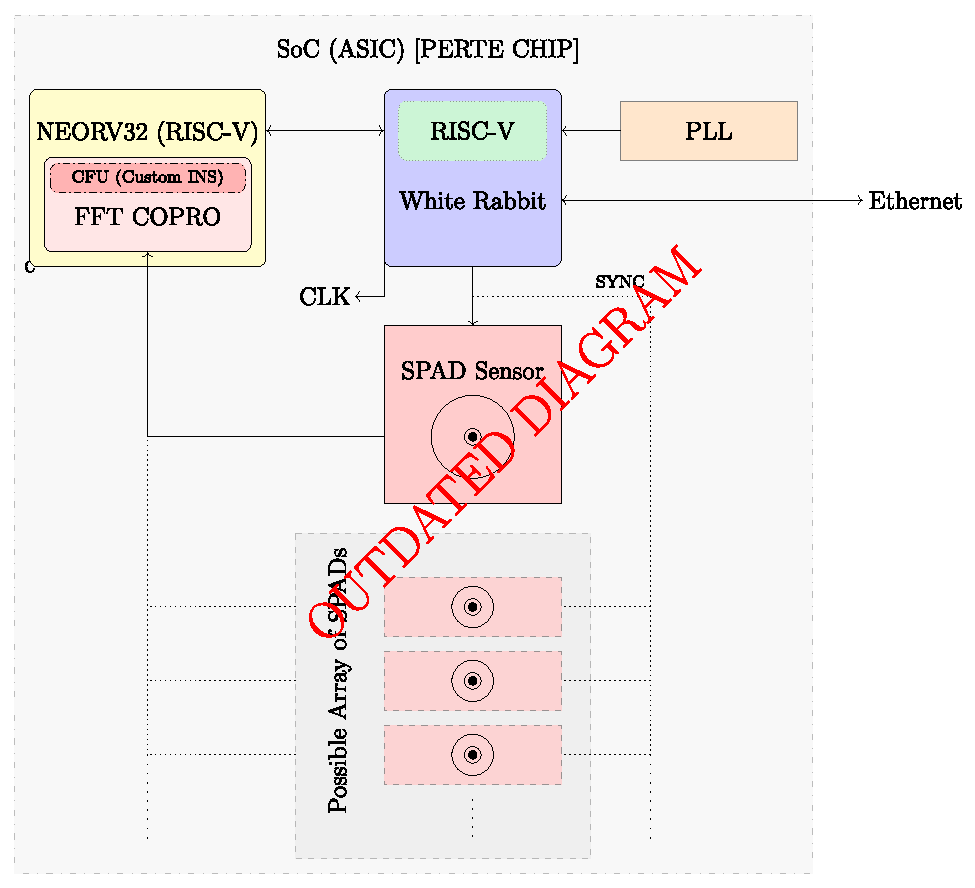
\includegraphics[width=14cm]{figures/ASIC-Diagram.pdf}
    \caption{ASIC to be develop.}
    \label{fig:ASIC}
\end{figure}

\newpage 
\section{Contributions}
\label{contrib}

\noindent The PhD student Unai Sainz Estebanez has made the following contributions to Open Hardware Repository \cite{ohwr}.

\vspace{5mm}

\noindent In the \href{https://gitlab.com/ohwr/project/urv-core}{urv-core} repository (December 19, 2024):

\begin{itemize}
\item Three commits:
    \begin{itemize}
    \item \href{https://gitlab.com/ohwr/project/urv-core/-/commit/655d46fe9fcb8a0880f63734f613a1f863b340ec}{655d46fe9fcb8a0880f63734f613a1f863b340ec}
    \item \href{https://gitlab.com/ohwr/project/urv-core/-/commit/d311497ac22b0164953fc0eb7474a97620c819e2}{d311497ac22b0164953fc0eb7474a97620c819e2}
    \item \href{https://gitlab.com/ohwr/project/urv-core/-/commit/46a6842f953cfab5f1814b8f09324b6f739e133f}{46a6842f953cfab5f1814b8f09324b6f739e133f}
    \end{itemize}
\end{itemize}

\noindent Related issue: \footnote{Since the migration from \say{ohwr.org} to \say{gitlab.com}, the authors of the issues created on the old site have been aliased by the person who performed the migration.}

\vspace{5mm}

\href{https://gitlab.com/ohwr/project/urv-core/-/issues/10}{gitlab.com/ohwr/project/urv-core/-/issues/10}

\vspace{5mm}

\noindent In the \href{https://gitlab.com/ohwr/project/general-cores/}{general-cores} repository (February 3, 2025):

\begin{itemize}
\item One commit:
    \begin{itemize}
    \item \href{https://gitlab.com/ohwr/project/general-cores/-/commit/4f887ca87620116b199a898599c70c69b0f0b5f0}{4f887ca87620116b199a898599c70c69b0f0b5f0}
    \end{itemize}
\end{itemize}

\noindent Related issue:

\vspace{5mm}

\href{https://gitlab.com/ohwr/project/general-cores/-/issues/57}{gitlab.com/ohwr/project/general-cores/-/issues/57}

\vspace{5mm}

\noindent In the \href{https://gitlab.com/ohwr/project/wr-cores/}{wr-cores} repository (February 13, 2025):

\begin{itemize}
\item One commit:
    \begin{itemize}
    \item \href{https://gitlab.com/ohwr/project/wr-cores/-/commit/c940635009eff0e417f9b547fbd73396f89e6627}{c940635009eff0e417f9b547fbd73396f89e6627}
    \end{itemize}
\end{itemize}

\noindent Related issue:

\vspace{5mm}

\href{https://gitlab.com/ohwr/project/wr-cores/-/issues/102}{gitlab.com/ohwr/project/wr-cores/-/issues/102}

\vspace{5mm}

\noindent In the \href{https://gitlab.com/ohwr/project/gn4124-core/}{gn4124-core} repository (February 14, 2025):

\begin{itemize}
\item Three commits:
    \begin{itemize}
    \item \href{https://gitlab.com/ohwr/project/gn4124-core/-/commit/eef550ec1e227704af35739ff2168e80eda70d75}{eef550ec1e227704af35739ff2168e80eda70d75}
    \item \href{https://gitlab.com/ohwr/project/gn4124-core/-/commit/b1fe3889dfffbf3f6b40f8a46886a659de09fbc7}{b1fe3889dfffbf3f6b40f8a46886a659de09fbc7}
    \item \href{https://gitlab.com/ohwr/project/gn4124-core/-/commit/71c4d362442ad11ddd2b1fd7fd4d8ab1e1947a89}{71c4d362442ad11ddd2b1fd7fd4d8ab1e1947a89}
    \end{itemize}
\end{itemize}

\noindent Related issue:

\vspace{5mm}

\href{https://gitlab.com/ohwr/project/wr-cores/-/issues/101}{gitlab.com/ohwr/project/wr-cores/-/issues/101}


\clearpage % If you want the references in a separate page
\bibliography{bibliography}

%\clearpage % If you want the appendix in a separate page
%\appendix
%\input{sections/appendix}

\end{document}
